\section{Local Regulation}

To maintain good line regulation, the circuitry of the power supply is itself
powered by a local regulator.

\begin{figure}[H]
\centering
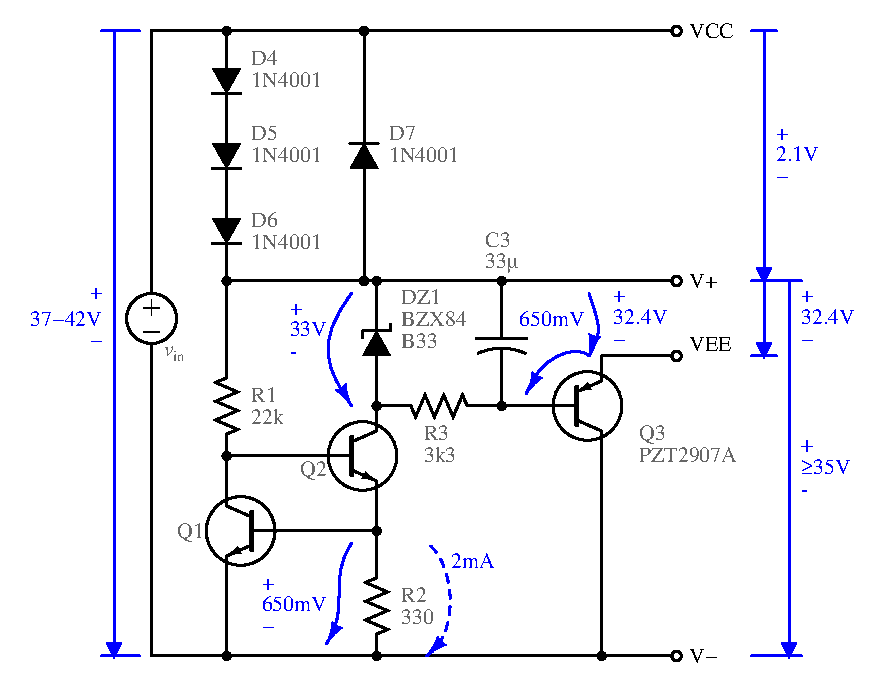
\includegraphics[width=5.5in]{sch/localregs}
\caption{Local regulator sub-schematic}
\label{fig:localreg}
\end{figure}

\begin{multicols}{2}

Note that unlike many electronic designs, this power supply uses a
\emph{positive ground} configuration. This means that rather than having
a higher voltage rail regulated with respect to a lower rail, the lower rail
is regulated to the higher one.

\subsubsection{VCC/V+ Auxiliary Rail}
A small positive rail is required about 2~V above ground to provide extra
headroom for the regulating circuits. The low current (500~mA) output means
that it is reasonably efficient to achieve this by passing the positive
supply input through a string of three diodes (0.7~V each, 2.1~V total), and
using the voltage appearing at the negative end as `ground', labeled V+ in the
circuit diagrams.
The voltage at the positive end is VCC.

This simple three-diode chain could barely be given the title ``voltage
regulator'', but it is used for this purpose.
Diode \texttt{D7}, connected backwards across the chain, protects the power
supply if an external voltage is applied to it while it is shut down. This
diode allows that external voltage to actually power the regulation circuitry,
protecting it from damage by reverse voltages.
\ \\

\subsubsection{VEE/V+ Primary Rail - Reference}
The VEE regulator is more complicated.

\texttt{Q1} and \texttt{Q2} act as a simple constant current source.
Consider what will happen
as the circuit starts up. The power switch will have just been flipped, and the
rails, once all equal in voltage, begin to drift apart.
\texttt{Q1} has \texttt{R2} pulling its base and
emitter together, so it begins turned off, and we can ignore it.
\texttt{Q2} has \texttt{R1} supplying it base current from V+, so it will
turn on. As V+ climbs, so does the current flowing through \texttt{Q2}, and
this same current flows through \texttt{R2}. Ohm's Law gives the voltage
across this resistor as equal to the product of the current and the resistance.
A typical transistor's threshold voltage is 650~mV. At this voltage, there is
$\frac{V}{R} = \frac{650\;mV}{330\;\Omega} = 1.97\;mA$ flowing. Because the
threshold voltage has been reached between \textrm{Q1}'s base and emitter,
\textrm{Q1} begins to turn on, diverting away \textrm{Q2}'s base current and
limiting the output current. This feedback action causes the current drawn
into \texttt{Q2} to settle at 1.97~mA.

\subsubsection{Primary Rail Regulation Tolerance}
Both the nominal 650~mV threshold voltage and the 330~$\Omega$ resistance
vary with temperature. The specified operating range of this power supply
is from 5~\dg C to 45~\dg C. The transistor's threshold voltage loses about
2~mV for every 1~\dg C above a standard 25~\dg C room temperature. 
A typical resistor might have a temperature coefficient of 200~ppm/\dg C,
or more properly, 200~($\mu\Omega$/$\Omega$)/\dg C,
meaning its resistance changes by 200~$\mu\Omega$ for every 1~$\Omega$
of its nominal value per 1~\dg C above the standard 25~\dg C.
This means that, assuming the threshold is indeed 650~mV at room temperature,
the temperature-dependent current drawn is:
\small
\begin{align*}
    & \textrm{Where } \Delta T = T - 25\;^\circ C\\
    &I(\Delta T) = \frac{V(\Delta T)}{R(\Delta T)} \\
    &\quad= \frac{650\;mV - (2\;mV/^\circ C)(\Delta T)}
      {(330\;\Omega)((200\;\mu\Omega/\Omega/^\circ C)(\Delta T) + 1)} \\
\end{align*}
\normalsize

This has its maximum value at the minimum value of $\Delta T$:
\small
\begin{align*}
    &I(-20^\circ C) = \frac{690\;mV}{328.68\;\Omega} = 2.10\;mA \\
\end{align*}
\normalsize

The error is $2.10\;mA - 1.97\;mA = 130\;\mu A$.

This 2~mA is drawn through \texttt{DZ1}, a BZX84-series, 2~\%-tolerance, 33~V
Zener diode, and this is precisely the current specified for the 2~\% tolerance.
The dynamic impedance (apparent output resistance at a specific bias point) of
\texttt{DZ1} is specified by the datasheet to be at worst 80~$\Omega$,
so the above
130~$\mu$A current error will cause a voltage error up to the product of the
two values:
$(130~\mu A)(80\;\Omega) = 10.4\;mV$, or 0.03~\% on top of the existing
2~\% tolerance. Further
error will be caused by \texttt{DZ1}'s temperature coefficient, given as
800ppm/\dg C: 1.6~\% in either direction over the specified range.
Assuming the temperature change is not enough to affect the dynamic
impedance, the errors can be added together, so
the total
non-trimmable voltage error is 1.6~\% + 0.03~\% = 1.63~\%. (The 2~\% is not
considered because it is constant --- a property of the individual diode ---
and can be adjusted with a trimmer).

\subsubsection{Primary Rail - Filter and Buffer}

The output voltage is filtered by \texttt{R3} and \texttt{C3}, a first-order
low pass filter with a cutoff frequency
$f_c = 1/(2\pi R_3 C_3) = 1.46\;Hz$ to filter out line ripple.
This is then buffered by \texttt{Q3}, a simple emitter-follower,
which loses about 650~mV: from -33~V to -32.35~V. It will have a 2~mV/\dg C
error just like \texttt{Q1}, contributing an additional 0.1~\% error, for a
grand total of 3.73~\%. There will be a slight, additional error in this
650~mV caused by self-heating and by load current, but this error is nearly
constant and will be calibrated away by the trimmers.

\end{multicols}
